\chapter{The 4+ Windows}%
\label{cha:the_4_windows}

\section{Program Window}%
\label{sec:program_window}

The main window is called the Program window and contains the timeline as well as the entry point for all menu driven operations.  
It is often just called the “timeline”.  
The timeline consists of a vertical stack of tracks with a horizontal representation of time. 
This defines the output of rendering operations and what is saved when you save files. 
To the left of the timeline is the patchbay which contains options affecting each track.  
The patchbay is described in detail in the Editing section.

The \emph{Window} pulldown on this main window contains options that affect the 4 main windows. 
\emph{Default} positions repositions all the windows to a 4 screen editing configuration.
On dual headed displays,
the Default positions operation fills only one monitor with windows.

\subsection{Video and Audio Tracks and Navigation}%
\label{sub:video_and_audio_tracks_and_navigation}

The program window (figure~\ref{fig:pathbay})   contains many features for navigation and displays the timeline as it is structured in memory: tracks stacked vertically and extending across time horizontally. 
The horizontal scroll bar allows you to scan across time. 
The vertical scroll bar allows you to scan across tracks.

\begin{figure}[htpb]
    \centering
    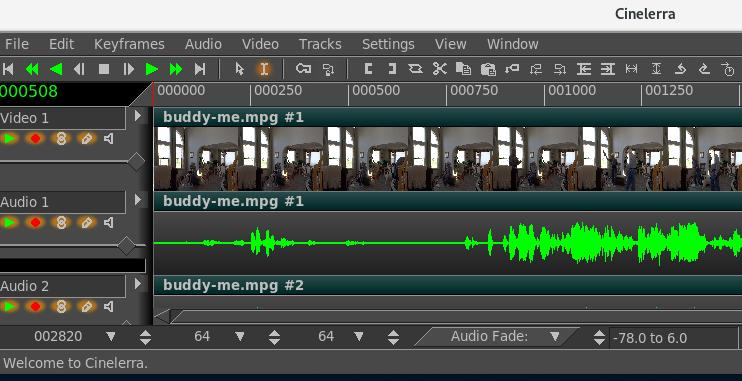
\includegraphics[width=0.8\linewidth]{images/pathbay.png}
    \caption{Patchbay  | Timeline with pulldowns \& navigation icons, Video/Audio tracks \& bottom Zoom}
    \label{fig:pathbay}
\end{figure}


Video tracks represent the duration of your videos and clips, just as if you placed real photographic film stock end-to-end on a table. 
The individual images you see on the track are samples of what is located at that particular instant on the timeline.

Audio tracks represent your sound media as an audio waveform. 
Following the film analogy, it would be as if you "viewed" magnetic tape horizontally on your table. 
You can adjust the horizontal and vertical magnification of the tracks and the magnification of the audio "waveform" display using the zoom panel controls. 
Every track on the timeline has a set of attributes on the left, called the patch- bay. 
It is used to control some of the behavior of the tracks.

Track Navigation involves both selecting a specific audio or video track and moving to a certain time in the track. 
The vertical scroll bar allows you to scan across tracks. 
For vertical scrolling you can also use the mouse wheel. 
The horizontal scroll bar allows you to scan across time. For horizontal scrolling you can use the mouse wheel with the Ctrl key.  

In addition to the graphical tools, you can use the keyboard to navigate.  
There is a shortcuts document for keyboard navigation; it includes, for example, shortcuts like use the Home and End keys to instantly go to the beginning or end of the timeline.  
Or in the default cut and paste mode, hold down Shift while pressing Home or End in order to select the region of the timeline between the insertion point and the key pressed.

\subsection{Zoom Panel}%
\label{sub:zoom_panel}

Below the timeline, you will find the zoom panel. 
The zoom panel contains values for sample zoom (duration visible on the timeline), amplitude (audio waveform scale), track zoom (height of tracks in the timeline), and curve zoom (automation range). 
In addition to the scrollbars, these zooms are the main tools for positioning the timeline.  
Also on the zoom panel is selection change and alpha slider.

\begin{figure}[htpb]
    \centering
    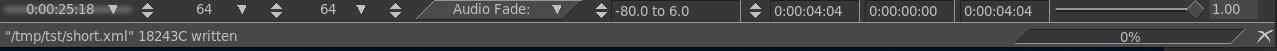
\includegraphics[width=0.99\linewidth]{images/zoompanel.png}
    \caption{Zoom panel on the bottom of the main program window}
    \label{fig:zoompanel}
\end{figure}

Changing the \emph{sample zoom} causes the unit of time displayed in the timeline to change size. 
It allows you to view your media all the way from individual frames to the entire length of your project. 
The higher the setting, the more frames you can see per screen. 
The sample zoom value is not an absolute reference for the unit of time since it refers to the duration visible on the timeline and thus changes also as you modify the length of the program window horizontally.
Use the Up and Down arrows to change the sample zoom by a power of two. 
Or if your mouse has a wheel, mouse over the tumblers and use the wheel to zoom in and out.


The \emph{amplitude} only affects audio which determines how large the waveform appears. Ctrl-up and Ctrl-down cause the amplitude zoom to change.

The \emph{track zoom} affects all tracks. 
It determines the height of each track. 
If you change the track zoom, the amplitude zoom compensates so that the audio waveforms look proportional. 
Ctrl-pgup and Ctrl-pgdown cause the track zoom to change.

The \emph{curve zoom} affects the curves in all the tracks of the same type. 
It determines the value range for curves. 
First select the automation type (audio fade, video fade, zoom, X,Y) then use the left tumblers for the minimum value and the right tumblers for the maximum value or manually enter the values in the text box. 
Normally you will use -40.0 to 6.0 for audio fade and 0.0 to 100.0 for video fade. 
The tumblers change curve amplitude, but the only way to curve offset is to use the fit curves button.

The \emph{selection start time}, \emph{selection length}, and \emph{selection end time} display the current selected timeline values.  
The \emph{alpha slider} allows for varying the alpha value when using colors on the tracks as set in your appearance preferences for Autocolor assets.  
It has no function without that flag set.

\subsection{Track Popup Menu}%
\label{sub:track_popup_menu}

Each Track has a popup menu. 
To activate the track popup menu, Right mouse click on the track. 
The popup menu affects the track whether the track is armed on the patchbay or not. 
The Track Menu contains a number of options:

\begin{description}
    \item[Attach Effect] opens a dialog box of effects applicable to the type of track of audio or video.
    \item[Move up] moves the selected track one step up in the stack.
    \item[Move down]  moves the selected track one step down in the stack.
    \item[Delete track]  removes the track from the timeline.
    \item[Add Track]  adds a track of the same media type, audio or video, as the one selected above that track.
    \item[Find in Resources]  that media file will be highlighted in the media folder in the Resources window.
    \item[Show edit]  will point out the exact start and stop points along with the length of the current edit on
        that track as well as the media name.
    \item[User title]  is used to change the title name.  This is really handy for files that have very long and
        similar names that would get cut off during edits.  You can use short names to better differentiate the
        media. If you select multiple, all those clips will have title name changed.
    \item[Bar color]  allows the user to select a specific color for the title bar.  This helps ease of locating.
    \item[Resize Track]  resizes the track.
    \item[Match Output Size]  resizes the track to match the current output size.
\end{description}


\subsection{Insertion Point}%
\label{sub:insertion_point}

The insertion point (figure~\ref{fig:insertion-points}) is the flashing hairline mark that vertically spans the timeline in the program window. 
Analogous to the cursor on your word processor, the insertion point marks the place on the timeline where the next activity will begin. 
It is the point where a paste operation takes place. 
When rendering, it defines the beginning of the region of the timeline to be rendered. It is also the starting point of all playback operations.
                           
Normally, the insertion point is moved by clicking inside the main timebar. 
Any region of the timebar not obscured by labels and in or out points is a hotspot for repositioning the insertion point. 
In cut and paste editing mode only, the insertion point can be moved also by clicking in the timeline itself. 
When moving the insertion point the position is either aligned to frames or aligned to samples. 
When editing video, you will want to align to frames. When editing audio you will want to align to samples. Select your preference by using Settings->Align cursor on frames.

\begin{figure}[htpb]
    \centering
    %\includegraphics[width=0.8\linewidth]{name.ext}
    \begin{tikzpicture}[scale=1, transform shape]
        \node (img1) [yshift=0cm, xshift=0cm, rotate=0] {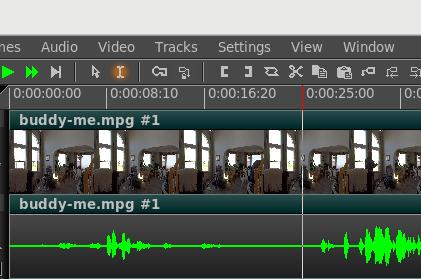
\includegraphics[width=0.6\linewidth]{images/insertion-point.png}};
        \node [yshift=-13mm, xshift=-1cm,anchor=east] at (img1.north west) (Pulldowns) {Pulldowns};
        \node [yshift=-20mm, xshift=-1cm,anchor=east] at (img1.north west) (Transport) {Transport \& Buttons Bar};
        \node [yshift=-27mm, xshift=-1cm,anchor=east] at (img1.north west) (Timebar) {Timebar};
        \node [yshift=-33mm, xshift=-1cm,anchor=east] at (img1.north west) (Title) {Media Title };
        \node [yshift=-43mm, xshift=-1cm,anchor=east] at (img1.north west) (Video) {Video Track};
        \node [yshift=-63mm, xshift=-1cm,anchor=east] at (img1.north west) (Audio) {Audio Track};
        \draw [->, line width=1mm] (Pulldowns) edge  ([yshift=-13mm] img1.north west);
        \draw [->, line width=1mm] (Transport) edge  ([yshift=-20mm] img1.north west);
        \draw [->, line width=1mm] (Timebar) edge    ([yshift=-27mm] img1.north west);
        \draw [->, line width=1mm] (Title) edge      ([yshift=-33mm] img1.north west);
        \draw [->, line width=1mm] (Video) edge      ([yshift=-43mm] img1.north west);
        \draw [->, line width=1mm] (Audio) edge      ([yshift=-63mm] img1.north west);
        \end{tikzpicture}
    
    \caption{Insertion point is at 0:00:25:10 in Hr:Mn:Sec:Frames}
    \label{fig:insertion-points}
\end{figure}


\subsection{Editing Modes}%
\label{sub:editing_modes}

There are 2 different editing methods of operation that affect the insertion point and the editing on the timeline.  
There is:  \emph{drag and drop mode} and \emph{cut and paste mode}. 
The editing mode is determined by selecting the arrow or the I-beam in the Transport and Buttons bar. 

If the arrow is highlighted, it enables \emph{drag and drop mode}.  
In drag and drop mode, clicking in the timeline does not reposition the insertion point.  
Double-clicking in the timeline selects the entire edit the mouse pointer is over.  
Dragging in the timeline repositions the edit the mouse pointer is over. 
This is useful for reordering audio playlists, sorting movie scenes, or moving effects around. 
To cut and paste in drag and drop mode you need to set in/out points to define an affected region. 

If the I-beam is highlighted it enables \emph{cut and paste mode}. 
In cut and paste mode, clicking in the timeline repositions the insertion point. 
Double-clicking in the timeline selects the entire edit the cursor is over. 
Dragging in the timeline highlights a region. 
The highlighted region becomes the region affected by cut and paste operations and the playback range during the next playback operation. 
Shift-clicking in the timeline extends the highlighted region.

When highlighting a region, the start and end points are either aligned to frames or aligned to samples. When editing video, you will want to align to frames. When editing audio you will want to align to samples. Select your preference by using settings->align cursor on frames.

\begin{figure}[htpb]
    \centering
    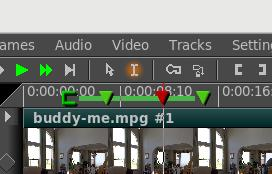
\includegraphics[width=0.4\linewidth]{images/i-beam.png}
    \caption{I-beam + in/out  +  labels}
    \label{fig:i-beam}
\end{figure}

\subsection{In/Out Points}%
\label{sub:in_out_points}

In both editing modes, you can set one In point and one Out point. 
The in/out points define the affected region. 
In drag and drop mode, they are the only way to define an affected region. 
In both cut and paste mode and drag and drop mode, the highlighted area overrides the In/Out points. 
If a highlighted area and In/Out points are set, the highlighted area is affected by editing operations and the In/Out points are ignored. 
If no region is highlighted, the In/Out points are used. 
To avoid confusion, it is better to use either highlighting or In/Out points but not both simultaneously.

To set in/out points, go to the timebar and position the insertion point somewhere. 
Select the In point button. 
Move the insertion point to a position after the In point and click the Out point button. 
Instead of using the button bar, you can use the [ or < and ] or > keys to toggle in/out points.

If you set the insertion point somewhere else while In/Out points already exist, when you click the In/Out buttons the existing points will be repositioned. 
If you click on in/out points while a region is highlighted, the insertion point will be ignored and In/Out points will be set at the beginning and at the end of the highlighted area.

If you select either the In point or the Out point, the insertion point will jump to that location. 
After selecting an In point, if you click the In point button the In point will be deleted. 
After selecting an Out point, if you click the Out point button the Out point will be deleted. 
Shift-clicking on an In/Out point highlights the region between the insertion point and that In/Out point. 
If a region is already highlighted, it extends the highlighted region up to that In/Out point.

To quickly get rid of In/Out points, without caring about where they are or if they are set or not, just double click on [ and ] buttons. 
The first click will set a new point or reposition an old one at the insertion point; the second click will delete it. This trick does not work if the In point or the Out point is already set at insertion point.

Some of the useful operations concerning the In/Out pointers are listed next.

\begin{description}
    \item[Ctrl-KeyPad\#]  if in/out set, KP 2,3,5,6 + Enter, play between In/Out point
    \item[Shift-Ctrl]  loops play between In/Out points
    \item[Click in/out] while holding the left mouse button, drags In/Out pointer elsewhere
    \item[Shift-Ctrl] with transport button, loops play between In/Out points
    \item[Ctrl-t]  clears both In/Out points
\end{description}

\subsection{Labels}%
\label{sub:labels}

The insertion point and the In/Out points allow you to define an affected region, but they do not let you jump to exact points on the timeline very easily. 
Labels are an easy way to set exact locations on the timeline that you want to jump to. 
When you position the insertion point somewhere and click the label button, a new label appears on the timeline. 
With label traversal you can quickly seek back and forth on the timeline.

No matter what the zoom settings are, clicking on the label highlights it and positions the insertion point exactly where you set the label. 
The lower case letter “L” is a shortcut for the label button.

Labels can reposition the insertion point when they are selected but they can also be traversed with the label traversal buttons. When a label is out of view, the label traversal buttons reposition the timeline so the label is visible. Keyboard shortcuts for label traversal are:

\begin{description}
    \item[Ctrl-left] repositions the insertion point on the previous label.
    \item[Ctrl-right] repositions the insertion point on the next label.
\end{description}

The Label folder in the Resources window lists the timestamp of every label. 
You can edit the label list and add a title for every item using the popup menu. 
To open the Label info dialog right click on the label icon in the Resources window or directly on the label symbol on the timebar. 
With labels you can also select regions:

\begin{description}
    \item[Shift-Ctrl-left] highlights the region between the insertion point and the previous label.
    \item[Shift-Ctrl-right] highlights the region between the insertion point and the next label.
    \item[Double-clicking] on the timebar between two labels highlights the region between the labels.	   
    \item[Shift-clicking] on a label highlights the region between that label and the insertion point.
        If a region is already highlighted, it extends the highlighted region up to that label.
\end{description}


If you hit the label button when a region is highlighted, labels are created at each end of the highlighted region. 
However, if one end already has a label, then the existing label is deleted. 
Hitting the label button again when a label is selected deletes it. 
Manually hitting the label button or L key over and over again to delete a series of labels can get tedious. 
To delete a set of labels, first highlight a region, then use the Edit->Clear labels function. 
If in/out points exist, the labels between the in/out points are cleared and the highlighted region is ignored.


In Cut and Paste editing mode only, by enabling \emph{Edit labels} in the settings menu or by disabling the \emph{Lock labels from moving} button on the program toolbar, labels will be cut, copied or pasted along with the selected region of the first armed track. 
Similarly, if a selected area of a resource is spliced from the viewer to the timeline in a position before labels, these labels will be pushed to the right on the timebar for the length of the selected area. 
To prevent labels from moving on the timebar, just disable the \emph{Edit labels} option or enable the \emph{Lock labels from moving} button.


Originally in Drag and Drop editing mode labels will be always locked to the timebar, even with the \emph{Edit labels} option enabled.  
This may no longer be correct in all cases. 

\subsection{Color Title Bars and Assets}%
\label{sub:color_title_bars_and_assets}

In order to visually aid in locating clips on the timeline that are from the same media file, you can have them auto-colored or self-colored.  
Use of this feature requires additional memory and cpu on every timeline redraw, therefore it is recommended that smaller computers leave it turned off.

For auto-color the color will be based on a hashed filename so that whenever you load this particular media, it will always have the same color on the title bar even if you use proxy.  
To enable auto-color (figure~\ref{fig:autocolor_assets}, go to Settings$\rightarrow$Preferences, Appearance tab and check on “Autocolor assets”.  
It is disabled by default.  
Each media will have a random muted color and there could easily be close duplicates as generated by the program algorithm.  There will be no total black, but some dark shades are possible.  

Screencast shows the red colored checkmark to enable Autocolor assets.  
In the lower left corner is Highlighting Inversion color which can also be set and is discussed elsewhere.

\begin{figure}[htpb]
    \centering
    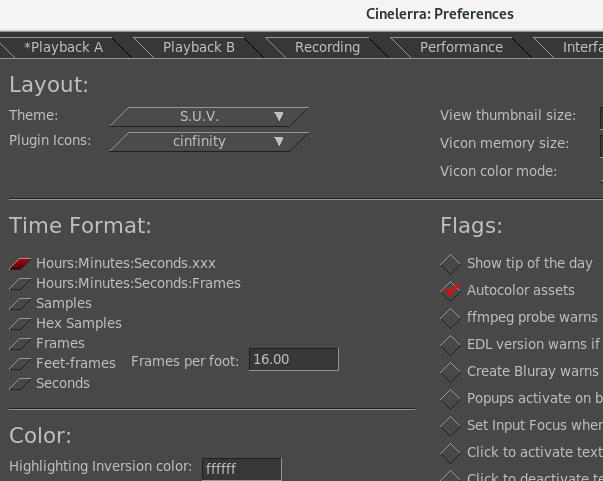
\includegraphics[width=0.8\linewidth]{images/autocolor-assets.png}
    \caption{Autocolor assets}
    \label{fig:autocolor_assets}
\end{figure}

To change a specific clip to your own chosen color, middle mouse button over that clip and an Edits popup will be displayed.  
Choose the option \emph{Bar Color} to bring up the color picker and choose a color.   
You can also change the alpha value in the color picker and this alpha takes precedence over the current alpha slider bar value unless it was set to 1.0.   
The color will only change after you click on the checkmark.  
The \emph{Bar Color} option works in either Drag and Drop or Cut and Paste editing mode and also works if “Autocolor assets” is not set.  
In Drag and Drop editing mode, if you select several clips and then bring up the Edits popup with the middle mouse button over a track, you can use the \emph{Bar Color} option to change all of those selected to the same color.

To go back to the default colors, uncheck “Autocolor assets” in Preferences, but this does not affect the specially chosen self-colored ones as they are preserved.  
To change these individually or  selectively use the Edits popup \emph{Bar Color} option and click on “Default” in the color picker window.  Auto-color does not honor armed/disarmed tracks.  
Self-color does honor armed/disarmed tracks.

And that’s not all!  
There is an \emph{alpha fader slider bar} on the bottom of the main window on the right hand side of what is referred to as the Zoom Panel.  
With this alpha slider, you can colorize your video and audio tracks to either see only the color at 0.0 or see only the image/audio waveform at 1.0.  
This slider bar affects all colored areas of the Autocolor assets and the self-colored ones.  
In the case when a specifically changed edit alpha value is any value except 1, the slider bar will not affect that.  
Once you use the slider bar, it is activated so gets first shot at any keystrokes in the main window.  
You deactivate this by simply clicking in a different part of the main window.  

As long as we are on the subject of color, just a reminder that you can also change the “Highlighting Inversion color” in Settings$\rightarrow$Preferences, Appearance tab.  
This is on right left hand side of the menu more than half the way down and you can see this in the figure~\ref{fig:autocolor_assets}.  
That setting defaults to white (ffffff) but sometimes this is a little bright so you can put any hex value in that suits you.

Screencast (figure~\ref{fig:autocolor_assets_alpha}a) which shows an example of the Autocolor assets with alpha set to 0.0.
In this screencast (figure~\ref{fig:autocolor_assets_alpha}b), the alpha is set to show the image as well as the colors.  The pink media file has been self-colored rather than the autocolor to make it easy to see.

\begin{figure}[htpb]
    \centering
    \begin{minipage}[h]{0.55\linewidth}
        \center{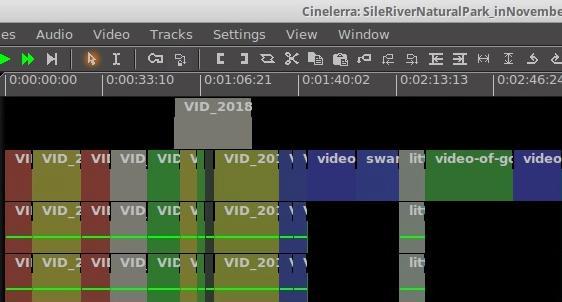
\includegraphics[width=0.99\linewidth]{images/autocolor-assets_alpha0.png}} \\ a)
    \end{minipage}
    \begin{minipage}[h]{0.4\linewidth}
        \center{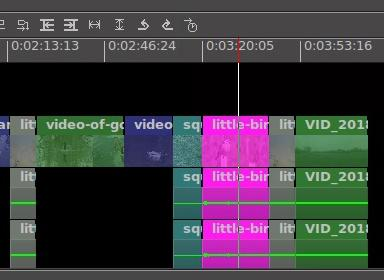
\includegraphics[width=0.99\linewidth]{images/autocolor-assets_alpha1.png}} \\ b)
    \end{minipage}
    \caption{An example of the Autocolor assets}
    \label{fig:autocolor_assets_alpha}
\end{figure}


\subsection{More about Pulldowns}%
\label{sub:more_about_pulldowns}

The main window pulldowns are quite obvious in their meaning and usage, so here is only a summary.  
%TODO Figure 3 shows an example of the pulldowns as displayed in the main window.


\begin{description}
    \item[File]  options for loading, saving, and rendering as described in other sections.
    \item[Edit]  edit functions; most of which have shortcuts that you will quickly learn.
    \item[Keyframes]  keyframe options which are described in the Keyframe section.
    \item[Audio]  audio related functions such as “Add track”, “Attach transition/effect”.
    \item[Video]  video functions such as “Default/Attach transition”.
    \item[Tracks]  move or delete tracks are the most often used.
    \item[Settings]  this is mostly described in other sections.  
        However, typeless keyframes are not described
        anywhere else.  
        They allow keyframes from any track to be pasted on either audio or video tracks.
    \item[View]  for display or modifying asset parameters and values to include Fade, Speed, and Cameras.
    \item[Window]  window manipulation functions.
\end{description}


\subsection{Window Layouts}%
\label{sub:window_layouts}

If you like to use different window layouts than the default for certain scenarios, you can setup, save, and load 4 options.   
First position your Cinelerra windows where you want them to be and then use the Window pulldown and choose \emph{Save layout}.  
To use the default name of Layout \#, when the popup comes up, just click the green checkmark OK on the Layout popup menu.  
If you would like a specific name for your layout so you can remember what it is for, keyin 1-8 english characters that are meaningful to you (english characters mean you can not use the German umlaut or the French accent).  
Legal characters are a-z, A-z, 0-9, \_ (the underscore character) and a limit of 8 total.  
If you keyin more than 8, only the last 8 characters will be used.  
To rename a currently existing layout, use the Save layout option again on the one to rename, and keyin a different name into the text box or blank for the default name (figure~\ref{fig:window_layouts}).

\begin{figure}[htpb]
    \centering
    \begin{minipage}{.49\linewidth}
        \center{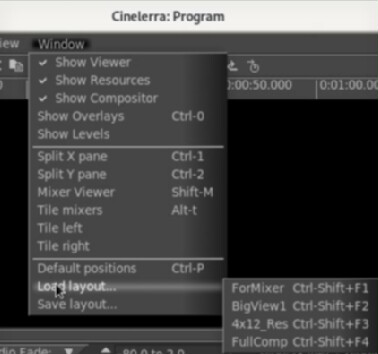
\includegraphics[width=1\linewidth]{images/window_layout1.png}}\\ a)
        %TODO High res image replace
    \end{minipage}
    \begin{minipage}{.49\linewidth}
        \vspace{13ex}
        \center{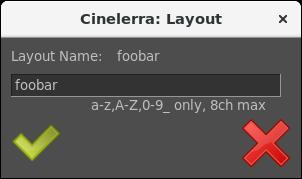
\includegraphics[width=1\linewidth]{images/window_layout2.png}}\\ b)
        %TODO Alpha channel
    \end{minipage}
    \caption{Window Layouts}
    \label{fig:window_layouts}
\end{figure}

The files containing the coordinates for your layouts will automatically be saved in the \texttt{\$HOME/.bcast} directory as \texttt{layout\#\_rc} or \texttt{layout\#\_8chars\_rc}.

To use the desired layout, keyin the shortcut or use the Window pulldown and choose \emph{Load layout} and then make your choice. 

\subsection{Just Playing!}%
\label{sub:just_playing_}
What if you are just using Cinelerra to play media and listen to tunes? 
After loading your media, just hit the space bar to start playing and then again to stop playing.  
Other than that, use the transport buttons on the top bar of the Program window.  
Other ways, not previously mentioned to “play around” are described next. 

\subsubsection*{Repeat Play / Looping Method}%
\label{ssub:repeat_play_looping_method}

There are 2 methods for repeat play or looping on the timeline and 1 method for both the Compositor and the Viewer.  This works in conjunction with any of the transport buttons or shortcuts in either forward or reverse as usual.  The 1 exception is that the Shift button can not be used to either add or subtract audio within the repeat area.


\emph{Shift-L on the Timeline}, repeats the selection per the algorithm outlined next.  
When setup, long green lines are displayed across the entire set of tracks which shows the start and end of the loop.
\begin{enumerate}
    \item  Highlighted selection repeats loop and takes precedence over all other possibilities.  
        If the cursor is before the highlighted area, it will play up to the area and then repeat the highlighted section.  
        If the cursor is after the highlighted section, play will start at the beginning until you get to the
        highlighted section and then repeat.
    \item  When both In and Out pointers are set, it repeats the section between [ and ].
    \item  If only one of the In or Out pointers is set, it loops the whole media.
\end{enumerate}

\emph{Ctrl+Shift+transport button on the Timeline, Viewer, and Compositor}

\begin{enumerate}
    \item Repeats entire media if no In or Out pointer set.
    \item  In and Out pointer set, repeats area between pointers.
    \item  Only In pointer set, repeats from In to end of media.
\end{enumerate}

\subsubsection*{Last Play Position Memory}%
\label{ssub:last_play_position_memory}


When you play media, the start/end playback positions are saved as if they had been made into temporary labels.  
They appear on the timeline as purple/yellow hairline markers representing the last start/end labels for the last playback. 
They can be addressed as if they are label markers using:

\begin{description}
    \item[Ctrl$\leftarrow$]   tab to the label before the cursor, that is “play start”
    \item[Ctrl$\rightarrow$]   tab to the label after the cursor, that is “play stop”
\end{description}


You can use these markers for re-selection.  
Additionally, the selection region can be expanded by “pushing” the markers using single frame playback.  
Use frame reverse (keypad 4) to push the start play marker backward, or use frame forward (keypad 1) to push the end play marker forward.

Another handy feature is to use the combination of Ctrl-shift-arrow (left or right) to select the media from the cursor position (red hairline) to the start or end marker by “tabbing” to the label markers.  
For example, tab to the beginning of the previous play region using Ctrl-left-arrow to move the cursor to the beginning of last play, then press Ctrl-Shift-right-arrow to tab to the end of the playback region. 
Now you can clip/play/expand or edit the previous playback selection.

\begin{description}
    \item[Ctrl SHIFT$\rightarrow$] 	  tab cursor to label right of cursor position and expand selection
    \item[Ctrl SHIFT$\leftarrow$] 	  tab cursor to label left of cursor position and expand selection
\end{description}


\subsubsection*{Playback Speed Automation Support}%
\label{ssub:playback_speed_automation_support}


The speed automation causes the playback sampling rate to increase or decrease to a period controlled by the speed automation curve.  
This can make playback speed-up or slow-down according to the scaled sampling rate, as “time is multiplied by speed” (speed X unit\_rate).

\subsubsection*{Alternative to using Numeric Keypad for Playing}%
\label{ssub:alternative_to_using_numeric_keypad_for_playing}


For the keyboards without a numeric keypad or if you prefer to use keys closer to where you normally type, there are alternative keys for the play/transport functions.  These are listed below.

\begin{tabular}{lcl}
	Alt + m&=&stop playback\\

	Alt + j&=&forward single frame\\

	Alt + k&=&forward slow playback\\

	Alt + l&=&forward normal playback\\

	Alt + ;&=&forward fast playback\\

	Alt + u&=&reverse single frame\\

	Alt + i&=&reverse slow playback\\

	Alt + o&=&reverse normal playback\\

	Alt + p&=&reverse fast playback\\
\end{tabular}
\begin{minipage}{.45\linewidth}
+ Shift key, results in the reverse of whether audio is included or not.
\vspace{1ex}

+ Ctrl, results in the transport function operating only between the in/out pointers.
\end{minipage}

\section{Compositor Window}%
\label{sec:compositor_window}

The Compositor window (figure~\ref{fig:compositor_window}) displays the output of the timeline. 
It is the interface for most compositing operations or operations that affect the appearance of the timeline output. 
Operations done in the Compositor affect the timeline but do not affect clips.

\begin{figure}[htpb]
    \centering
    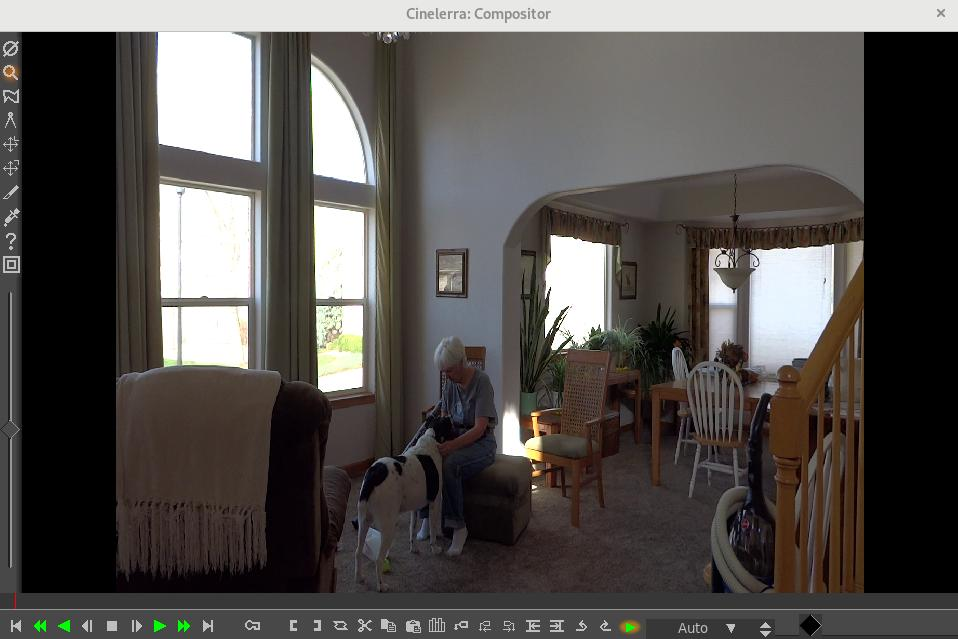
\includegraphics[width=0.8\linewidth]{images/compositor_window.png}
    \caption{Upper right side contains navigation tools / bottom bar has manu control functions}
    \label{fig:compositor_window}
\end{figure}

\subsection{Compositor controls}%
\label{sub:compositor_controls}


Navigating the video output does not affect the rendered output; it just changes the point of view in the compositor window. 
The video output has several navigation functions. 
The video output size is either locked to the window size or unlocked with scrollbars for navigation. 
The video output can be zoomed in and out and panned. 
If it is unlocked from the window size, middle clicking and dragging anywhere in the video pans the point of view. Hitting the + and - keys zooms in and out of the video output.

Underneath the video output are copies of many of the functions available in the main window. 
In addition there is a zoom menu and a tally light. 
The zoom menu jumps to all the possible zoom settings and, through the Auto option, locks the video to the window size. 
The zoom menu does not affect the window size. 
The tally light turns red when rendering is happening. This is useful for knowing if the output is current. 
Right clicking anywhere in the video output brings up a menu with all the zoom levels, zoom auto mode, and some other options. 
In this particular case the zoom levels resize the entire window and not just the video. 
The \emph{Reset camera} and \emph{Reset projector} options center the camera and projector. 
The \emph{Hide controls} option hides everything except the video. 

On the left of the video output is a toolbar specific to the compositor window. The toolbar has the following functions:

\emph{Protect video} --- disables changes to the compositor output from clicks in it. It is an extra layer on top of the track arming toggle to prevent unwanted changes.

\emph{Magnifying glass} --- this tool zooms in and out of the compositor output without resizing the window. If the video output is currently locked to the size of the window, clicking in it with the magnifying glass unlocks it and creates scrollbars for navigation.

\begin{description}
    \item[ Left clicking] in the video zooms in;
    \item[Ctrl clicking] in the video zooms out;
    \item[Rotating the wheel] on a wheel mouse zooms in and out.
\end{description}

In addition, if you enable the Magnifying glass, a zoom slider for fine-viewing appears below these tools.  It allows you to zoom to most any size. A “zoom slider” will pop-up towards the bottom on the left-hand side of the Compositor when you enable “Zoom view” via the magnifying glass or when you click on the icons for “Adjust camera automation” or “Adjust projector automation”.  This will allow for adjusting the amount of zoom at any level between .01 and 100 based on a logarithmic scale.  When using the zoom slider, the number by which the view is zoomed can be seen in the textbox where the original-also-working % zoom is located.  The zoom slider size is in the form of “times”, such as x 0.82 which indicates that the picture is zoomed to 82/100th of the original size as seen in Settings→Format.  Once you have set the zoom to the desired size, use the vertical and horizontal scroll bars to position the view as needed.

